\documentclass{sig-alternate}

\usepackage{comment}

\newtheorem{mydef}{Definition}
\newtheorem{mylem}{Lemma}
\newtheorem{mythm}{Theorem}
\newtheorem{myprop}{Property}
\newtheorem{mycoro}{Corollary}

\begin{document}
	
% --- Author Metadata here ---
\conferenceinfo{GECCO'15,} {July 11-15, 2015, Madrid, Spain.}
\CopyrightYear{2015}
\crdata{TBA}
\clubpenalty=10000
\widowpenalty = 10000
% --- End of Author Metadata ---	

\title{Input-to-state stable analysis on Particle Swarm Optimization}
%\subtitle{[Extended Abstract]

\numberofauthors{3}

\author{
% 1st. author	
\alignauthor
Daqing Yi \\
%\affaddr{Computer Science Department}\\
\affaddr{Brigham Young University}\\
\affaddr{Provo, UT, USA}\\
\email{daqing.yi@byu.edu}
% 2nd. author	
\alignauthor
Kevin D. Seppi \\
%\affaddr{Computer Science Department}\\
\affaddr{Brigham Young University}\\
\affaddr{Provo, UT, USA}\\
\email{kseppi@cs.byu.edu}
% 3rd. author
\alignauthor
Michael A. Goodrich \\
%\affaddr{Computer Science Department}\\
\affaddr{Brigham Young University}\\
\affaddr{Provo, UT, USA}\\
\email{mike@cs.byu.edu}	
}

\maketitle

\begin{abstract}
This paper examines the dynamics of particle swarm optimization (PSO) by modeling PSO as a feedback cascade system and then applying input-to-state stability analysis.
Using a feedback cascade system model we can include the effects of the global-best and personal-best values more directly in the model of the dynamics.
Thus in contrast to previous study of PSO dynamics, the input-to-state stability property used here allows for the analysis of PSO both before and at stagnation.
In addition, the use of input-to-state stability allows this analysis to preserve random terms which were heretofore simplified to constants.
This analysis is important because it can inform the setting of PSO parameters and better characterize the nature of PSO as a dynamic system.
This work also illuminates the way in which the personal best and the global best updates influence the bound on particle's position and hence, how the algorithm exploits and explores the fitness landscape as a function of the personal best and global best.
\end{abstract}

\keywords{Particle Swarm Optimization, Input-to-state stability}

\begin{comment}
\emph{Input-to-state stable analysis} = 
Modeling by decomposition + Input-to-state stability
\begin{itemize}
\item Why input-to-state stable analysis is needed
    \begin{itemize}
    \item A better way of modeling PSO
    \item A better understand of the PSO dynamics
    \item Exploration + Exploitation (ISS)
    \item Match with the previous results
    \end{itemize}
\item When input-to-state stability is satisfied (Parameter selection)
    \begin{itemize}
    \item Input-to-state stability proof
    \item Moment analysis
    \end{itemize}
\item What happens when the position update of the particles are ISS
    \begin{itemize}
    \item Stagnation
    \item Beyond stagnation
    \end{itemize}
\end{itemize}

\end{comment}

\section{Introduction}
\label{sec:intro}
Particle Swarm Optimization (PSO) is a popular and well-studied algorithm that was originally motivated by the flocking behaviors of birds and insects.
Soon after its first publication it was discovered that the structure of the PSO algorithm is amenable to formal analysis using dynamical systems theory (sometimes referred to as dynamic systems) \cite{985692}.
The use of this theory has informed the setting of parameters \cite{Trelea2003317,Jiang20078}, lead to the proposal of new variants of the algorithm \cite{985692}, and allowed for the analysis of the behavior of the algorithm \cite{Schmitt:2013:PSO:2463372.2463563}, especially the behavior at stagnation, that is, when the algorithm fails to find better solutions \cite{985692}.

While the study of the algorithm at stagnation is important and a significant first step, it only answers questions about the behavior at the point that PSO has degenerated into random search.
At that point the algorithm can be mimicked by simply sampling from the appropriate distribution \cite{5175367}.
In this paper we extend the limited work that has been done to understand
the behavior \emph{before} stagnation, that is, when the unique mechanisms of PSO are directing the behavior of the algorithm.

By using a \emph{feedback cascade model} we are able to include both what we refer to as the \emph{position update} which comes from the PSO equations, but also the \emph{input update}, that is, the affect of the personal and global best.
This paper does so in contrast to prior work which focuses on the position update.
This model also allows us to make fewer assumptions in mapping from PSO to a dynamical system model.
Using the cascade model we are able to derive the conditions under which the process is input-to-state stable (ISS)\cite{Jiang2001857}, produce bounds on particle motion, as well as prove bounds on the mean of particle motion.
The ISS conditions and the bounds can inform parameter adjustments and other properties that can, in turn, control the extent to which the algorithm explores or exploits the fitness landscape.
This is espeically valuable in the context of the design of future PSO variants. 

The body of this paper is organized as described here.
In section \ref{sec:sys_model}, we model the PSO dynamics as a feedback cascade system, which enables the input-to-state stability analysis.
The definition of input-to-state stability (ISS) and how it means to the PSO is also given.
Section \ref{sec:iss} shows that for particular parameter values, the position update component of a particle is ISS. 
Using the ISS property we then give the bound on particle motion.
We also introduce how the ISS property applies to the moment analysis of the particle behavior.
In section \ref{sec:sys_dynamics}, we look at how the ISS helps analyzes the dynamics of the particle.
With the ISS property of the input update component, we could analyze the dynamics of the particle before and at stagnation.

\section{Related Work}
\label{sec:relwork}

Although the input-to-state stable analysis given in this paper can be applied to many versions of PSO,
for this work we use the formulas from Kennedy's most recent definition of PSO\cite{4223164}.
This version of PSO includes a star topology, and a constricted position update rule. 
The constricted position update rule is

\begin{subequations}
\label{eq:pso_alg}
\begin{equation}
\label{eq:up_vel}
\begin{aligned}
v_{ij}(k+1) & = \chi [ v_{ij}(k) 
+ \phi^{P} u^{P}_{ij}(k) (x^{P}_{ij}(k) - x_{ij}(k))
\\ & + \phi^{G} u^{G}_{ij}(k) ( x^{G}_{ij}(k) - x_{ij}(k)) ],
\end{aligned}
\end{equation}
\begin{equation}
\label{eq:up_pos}
x_{ij}(k+1) = x_{ij}(k) + v_{ij}(k+1).
\end{equation}
\end{subequations}
$ x_{ij}(k) $ represents the position of particle $ i $ in dimension $ j $ at time $ k $.
$ v_{ij}(k) $ similarly represents the velocity of particle $ i $ in dimension $ j $ also at time $ k $.
$ x^{G}_{ij}(k) $ and $ x^{P}_{ij}(k) $ are global (actually topology) and personal best positions observed by the swarm and the particle respectively. 
$ u^{G}_{ij}(k) $ and $ u^{P}_{ij}(k) $ are independent random values drawn from $ [0,1] $.
$ \chi \in ( 0, 1 ) $, $ \phi^{P} $ and $ \phi^{G} $ are algorithm parameters.

Due to the stochastic nature of the particle's path and the social interaction represented by the topology, the dynamics of the algorithm is hard to evaluate in general.
However once a particle is no longer able to find improvements in $ x^{G} $ and $ x^{P} $, it exhibits the \emph{stagnation phenomenon} \cite{Clerc06stagnationanalysis}.
In this state the analysis is easier since there is no effect from the topology.

Previous work that assumes stagnation can be categorized into two groups each based on how the analysis treats the stochastic factors.
The first approach is to ignore the stochastic factors.
Using this simplification, the convergence of a particle at stagnation can be analyzed \cite{985692}. 
By building a linear system model \cite{4424687}, the PSO algorithm can be viewed as a closed loop system and the convergence can be analyzed.
Based on such a convergence analysis, parameters can be set for best effect \cite{Trelea2003317}.

The second approach for handling the stochastic factors is based on the stochastic analysis.
By taking the mean of the stochastic variables, the stochastic terms can be converted into
constant terms.
A convergence analysis of the mean and variance of a particle at stagnation can also be obtained by using the characteristic equation in a discrete-time model 
\cite{Jiang20078}.
In a similar way, 
other moments can be computed
\cite{5175367,Poli:2007:EAS:1276958.1276977,Poli:2008:DSS:1384929.1384944}.
Using the discrete-time system model of different moments, the equilibrium can be found.
The stability requirements can be obtained from the norm by setting the root values of the characteristic equation to all be less than 1.

There is also some work that addresses the dynamics when a particle is not in the stagnation phase.
The discrete-time dynamics of PSO, that is, the dynamics of particle trajectory, can be approximated
using a continuous-time model
\cite{5675669}.
Furthermore, the probability of convergence in time can be analyzed
by viewing the update process as a random search process
\cite{vandenBergh:2010:CPP:2010420.2010421}.
The process of particles reaching a local optimum
has also been analyzed
\cite{Schmitt:2013:PSO:2463372.2463563}.

\section{Input-to-state stable analysis of the standard PSO}
\label{sec:sys_model}

The input-to-state stability analysis consists of two parts:
\begin{itemize}
\item how to decompose a system into components;
\item and the input-to-state stability of each component.
\end{itemize}
In this section, we model the particle into a feedback cascade model.
Then we review the definition of the input-to-state stability (ISS).
We also explain why the ISS should be applied into understanding the PSO.

\subsection{Feedback Cascade Model}
\label{sec:feedback_cascade_model}

In the purpose of input-to-state stability analysis, we model the system structure of a particle in PSO.
%This enables analysis of PSO with stochastic factors preserved and without the stagnation assumption.
As shown in Figure \ref{fig:sys_flow}, this system is comprised of cascaded component and feedback of the historical state.
These two components are the 
\emph{input update component} for the global best ($ x^{G}_{i}(k) $) and the personal best ($ x^{P}_{i}(k) $), and the 
\emph{position update component} for particle position ($ x_{i}(k+1) $), which depends on the inputs $ x^{G}_{i}(k) $ and $ x^{P}_{i}(k) $ as well as the last position $ x_{i}(k) $.

\begin{figure}
	\centering
	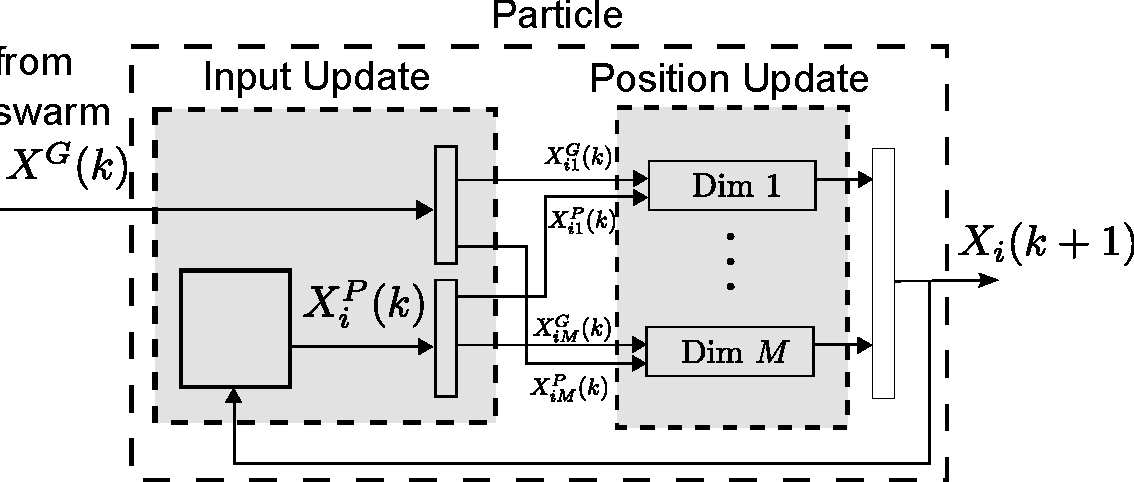
\includegraphics[width=0.5\textwidth]{particle_sys_flow.pdf}
	\caption{System structure of PSO}
	\label{fig:sys_flow}
\end{figure}

The properties of this system can be analyzed by using the input-to-state stability of the position update component and the input update component. 
Given an input-to-state stable position update component, we will see that the convergence of $ x_{i}(k) $ depends on bounds on $ x^{G}_{i}(k) $ and $ x^{P}_{i}(k) $.

\subsection{Input-to-state stability}
\label{sec:def_iss}

Before reviewing the definition of input-to-state stability, we first introduce several types of functions \cite{Jiang2001857}.
\begin{itemize}
	\item $ K $-function $ \mathbb{K} $ : a function $ \alpha  : [ 0, a ) \rightarrow [ 0, \infty ) $ is continuous, strictly increasing and $ \alpha (0) = 0 $; it is a $ K_{\infty} $-function, if $ \alpha (s) \rightarrow \infty $ as $ s \rightarrow \infty $;
	\item $ KL $-function $ \mathbb{KL} $ : a function $ \beta : [ 0, a ) \times [ 0 , \infty ) \rightarrow [ 0, \infty ) $ satisfies:
	\begin{enumerate}
		\item $ \forall t \geq 0 $, $ \beta (\cdot , t ) $ is a $ K $-function;
		\item $ \forall s \geq 0 $, $ \beta (s, \cdot) $ is decreasing and $ \beta(s,t) \rightarrow 0 $ as $ t \rightarrow \infty $.
	\end{enumerate}
	%\item Positive-definite function: a function $ \gamma (s) > 0, \forall s > 0 $ and $ \gamma (0) = 0 $.
\end{itemize}

We then have the definition of input-to-state stability in Definition \ref{def:iss}.

\begin{mydef}[Input-to-state stable]\cite{Jiang2001857}
\label{def:iss}
For a discrete-time system
\begin{equation}
\label{eq:dis_nonlinear}
x(k+1) = f( x(k) , u(k) ),
\end{equation}
with $ f(0,0) = 0 $
\footnote{This means that $ x = 0 $ is an equilibrium of the 0-input system.}, the system is \emph{(globally) input-to-state stable} if there exist a $ KL $-function $ \beta  $ and a $ K $-function $ \gamma $ such that, for each input $ u \in l^{m}_{\infty} $ and each $ \xi \in \mathbb{R}^{n} $, it holds that $  \forall k \in \mathbb{Z}^{+} $,
\begin{equation}
\label{eq:def_iss}
| x(k, \xi, u) | \leq \beta (| \xi |, k) + \gamma (\lVert u \rVert).
\end{equation}
\end{mydef}

The $ \beta () $ term in equation \eqref{eq:def_iss} defines an initial bound with a decaying property.
The $ \gamma () $ term in equation \eqref{eq:def_iss} defines a bound determined by the input.
This means that the influence $ \beta () $ term gradually decreases to zero and the position is bounded by a range determined by the bound on the input.

\subsection{The need of input-to-state stability in PSO}
\label{sec:connect_iss_to_pso}

Understanding the input-to-state stability of components in a system helps understanding the dynamics of a system.
By decomposing the PSO into several components, we could evaluate the input-to-state stability of each component separately. 
Because the parallel connection of input-to-state stable components reserves the input-to-state stable property.
As in Figure \ref{fig:sys_flow}, if each component of single dimension is input-to-state stable,  the position update component which combines all the dimension is still input-to-state stable.
We have property \ref{prop:iss:parallel}.
\begin{myprop}
\label{prop:iss:parallel}
The position update component is input-to-state stable if the update in each dimension is input-to-state stable.
\end{myprop}
This simplifies the analysis of the system by looking at only single dimension separately.
The serial connection and the feedback connection also lead to some interesting property from input-to-state stability, which will be discussed in Section \ref{sec:sys_dynamics}.

The input-to-state stability analysis also provides the tool to know the convergence and the boundary of the PSO.
PSO is designed to strike an effective balance between \emph{exploring} and \emph{exploiting} a fitness landscape.
A bound on a particle's state is an indicator of the nature of that balance.
When this bound is large the particle is exploring.
However, as a particle finishes exploring and reach stagnation, a particle's position should converge.

Input-to-state stability implies that the state of the system is bounded in a range determined by the bounds on the input.
Before stagnation, when the personal best and global best values have not converged, we can expect only looser bounds on the particle state.
These looser bounds reflect both what is know about the input and the what is know about the update process itself.

We call the bounds on the global best and personal best the ``exploit radius'' and the bounds on the particle's position a ``explore radius''.
The ratio of the explore radius to the exploit radius is determined by the parameters of the position update component.
However, if the personal best and global best converge to an estimated optimal position, the exploit radius falls to zero and the explore radius declines to a bound.

\begin{figure}
\centering
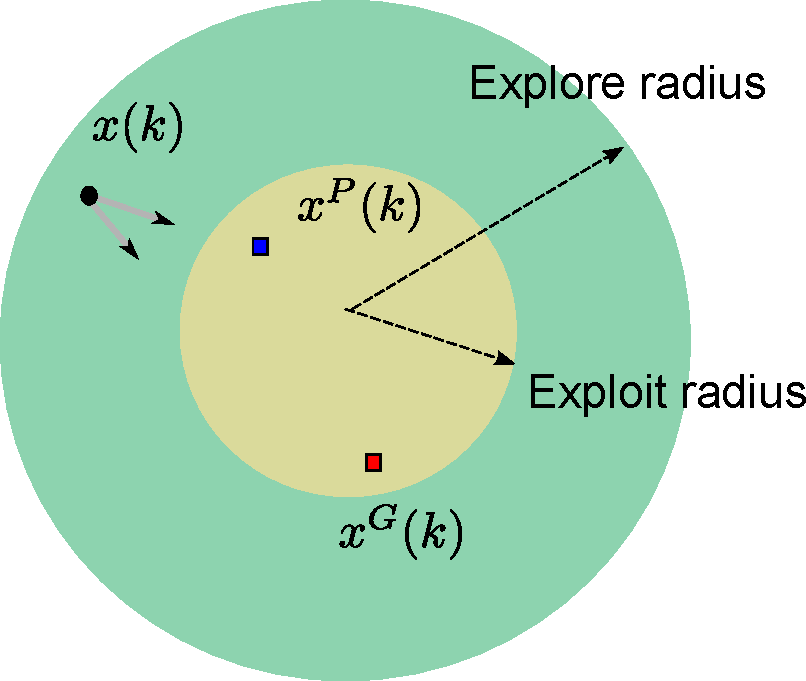
\includegraphics[width=0.6\linewidth]{./explore_and_exploit.pdf}
\caption{Exploration and exploitation.}
\label{fig:explore_and_exploit}
\end{figure}

\section{When the Input-to-state stability of PSO is satisfied (Parameter Selection)}
\label{sec:iss}

In this section, we briefly review the definition of input-to-state stability (ISS) including both the conditions that guarantee it and the bound that ISS implies\cite{Jiang2001857}. 
We then show that PSO satisfies this definition when the parameters of PSO are set in the requisite range. 
We also derive the bounds implied by the ISS property.
We use the ISS property in Section \ref{sec:sys_dynamics} to find bounds on particle motion.
We also introduce ISS into moment analysis.

In our analysis of the PSO algorithm, we seek to understand how the particles converge to some position $ x^{*} $, which is intended (not guaranteed) by the algorithm to be the optimal position.

We look at a one-dimension particle and extract the linear form of the position update component.
\begin{equation}
\label{eq:pso_up_linalg_simp}
X(k+1) = A(k) X(k) + B(k) U(k)
\end{equation}
with
$ A(k) = \begin{bmatrix}
\chi & - \chi \phi^{G} u^{G}(k) - \chi \phi^{P} u^{P}(k)
\\ 
\chi & 1 - \chi \phi^{G} u^{G}(k) - \chi \phi^{P} u^{P}(k)
\end{bmatrix} $
and
$ B(k) = \begin{bmatrix}
\chi \phi^{G} u^{G}(k) & \chi \phi^{P} u^{P}(k)
\\ 
\chi \phi^{G} u^{G}(k) & \chi \phi^{P} u^{P}(k)
\end{bmatrix} $.

The system state is $ X(k) = [ v(k), x(k) - x^{*} ]^{T} $, and the system input is $ U(k) = [ x^{G}(k) - x^{*} , x^{P}(k) - x^{*} ]^{T} $
\footnote{$ x^{*} $ means an equilibrium point to the system.
In PSO, it can be a local optimum, a global optimum, or an estimated optimum.
We use it as a reference point to check the bounds.}
.
The convergence of this model means that $ v(k) \rightarrow 0 $ and $ x(k) \rightarrow x^{*} $.

\subsection{Conditions for input-to-state stability for position update in PSO}
\label{sec:iss_proof}

Using the definition of the PSO position update as given in equation \eqref{eq:pso_up_linalg_simp}, PSO can be shown to be ISS as defined in definition \ref{def:iss}.

\begin{mythm}
\label{thm:iss}
The system \eqref{eq:pso_up_linalg_simp} is input-to-state stable, when $ | \lambda_{\max} ( A(k) ) | < 1 $.
%The system \eqref{eq:pso_up_linalg_simp} is input-to-state stable, if there exists a symmetric positive definite matrix $ P $ and a symmetric positive definite matrix $ Q' $ that has $ A(k)^{T} P A(k) - P = - Q(k) \leq - Q' $.
\begin{proof}
The proof follows the ISS-Lyapunov-function approach. 
The ISS-Lyapunov function, defined in Appendix \ref{sec:iss_lyapunov:func}, can be used to prove the input-to-state stability of a system and analyze the state bound\cite{Jiang2001857}.
The details of the proof is given in Appendix \ref{sec:thm:iss:proof}.
\end{proof}
\end{mythm}

Note that in using equation \eqref{eq:pso_up_linalg_simp},
$ [ v(k), x(k) - x^{*} ]^{T} = [0, 0]^{T} $ is an equilibrium position when the input $ [ x^{G}(k) - x^{*} , x^{P}(k) - x^{*} ]^{T} = [0, 0]^{T} $.
For an arbitrary optimization problem $ x^{*} $ would typically not be at the origin. 
In such a problem, input-to-state stability means that the boundaries of $ | v(k) | $ and $ | x(k) - x^{*} | $ would be transformed and thus determined by $ | x^{G}(k) - x^{*} | $ and $ | x^{P}(k) - x^{*} | $,
but the properties of ISS still apply independent of where the function is centered.

Having proven that PSO is ISS we can now state a bound on particle position.

\begin{mycoro}
\label{coro:state_bound}
Given the bound on the input $ || u || $ in the position update component, we have the bound on the particle position from equation \eqref{eq:pso_up_linalg_simp}.
\begin{equation}
\label{eq:state_bound}
\forall k, 
| x(k) - x^{*} | \leq \max ( | x(0) - x^{*} | , \gamma ( | [ x^{G}(k) - x^{*}, x^{P}(k) - x^{*} ]^{T} | ) ),
\end{equation}
in which $ \gamma = \alpha_{3}^{-1} \circ \sigma $.

The $ \max $ part is needed to account for the effect of the starting point, represented by the first parameter. Eventually the effect of the starting point no longer affects the system, formally:
\begin{equation}
\label{eq:state_bound:conv}
\exists T, \forall k \geq T, 
|  x(k) - x^{*} | \leq \gamma ( | [ x^{G}(k) - x^{*}, x^{P}(k) - x^{*} ]^{T} | ).
\end{equation}
\begin{proof}
This is obtained from Remark 3.7 in \cite{Jiang2001857} and by choosing $ P $ be a symmetric identity matrix.
Furthermore we drop the velocity part becuase $ | x(k) - x^{*} | \leq | [ v(k), x(k) - x^{*} ]^{T} | $.
\end{proof}
\end{mycoro}

Figure \ref{fig:boundary} gives an example on how a particle's boundary is determined by the personal best and global best.

\begin{figure}
\centering
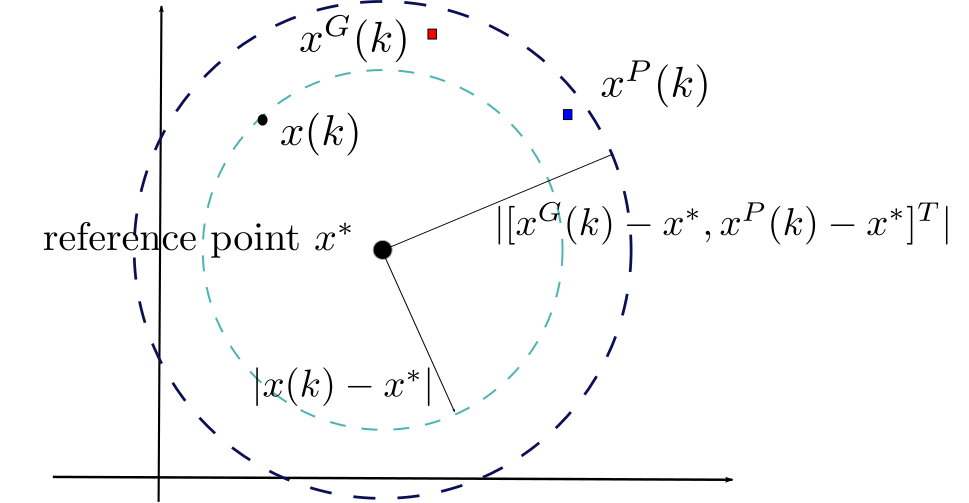
\includegraphics[width=0.8\linewidth]{./boundary}
\caption{A bound on a particle's position by a reference point $ x^{*} $ from Equation \ref{eq:state_bound:conv}.
The ratio of wo radii indicates $ \gamma $.}
\label{fig:boundary}
\end{figure}

\begin{mycoro}
\label{coro:param_unit_disc}
Write $ A(k) = 
\begin{bmatrix}
\chi & - \chi \phi \\
\chi & 1 - \chi \phi
\end{bmatrix}
$, in which
$ \phi \in [0,  \phi^{P} + \phi^{G} ] $ and $ \chi \in ( 0, 1 ) $.
When $ \phi \in (0 , \frac{2(1+\chi)}{\chi} ) $, the system \eqref{eq:pso_up_linalg_simp} is input-to-state stable.
\begin{proof}
The proof is given in Appendix \ref{sec:coro:param_unit_disc:proof}.
\end{proof}
\end{mycoro}

Figure \ref{fig:paramSpace} shows the parameter space.
The x-axis is $ \phi = \phi^{P} + \phi^{G} $ and the y-axis is $ \chi $.
The stable region in red is obtained from eigenvalue test on Theorem \ref{thm:iss} and the yellow boundary is obtained from Corollary \ref{coro:param_unit_disc}.
\begin{figure}
\centering
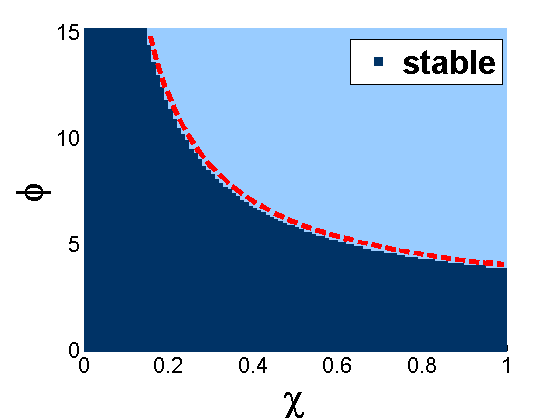
\includegraphics[width=0.7\linewidth]{./param2.png}
\caption{Parameter space}
\label{fig:paramSpace}
\end{figure}

\subsection{Moment Analysis}
\label{sec:moment_analysis}

Using the same perspective of the feedback cascade system, the input-to-stable stability analysis can also be applied to moment analysis.
Like the others \cite{Jiang20078,Poli:2008:DSS:1384929.1384944}, we derive the models on the statistical features on the particle's position.
The criteria for the convergence on the statistic values on the particle's position are given in \cite{Jiang20078} and \cite{Poli:2008:DSS:1384929.1384944}, when a particle is in stagnation.
The input-to-state stable analysis can provide the boundaries before reaching stagnation.

We adopt the approach of Jiang, Luo \& Yang to construct a model for the mean.
It is given that $ E( x(k) ) $ converges to $ \hat{x} = \frac{\phi^{P} x^{P} + \phi^{G} x^{G} }{ \phi^{P} + \phi^{G} } $ in stagnation \cite{Jiang20078}.
If we consider $ \hat{x} $ as a swarm average estimation on the optimum, we are interested in how $ E( x(k) ) $ deviates from $ \hat{x} $.
\begin{equation}
\label{eq:pso1_alg_mean_linalg:final}
\begin{aligned}
\begin{bmatrix}
E( x(k+1) ) - \hat{x} \\
E( x(k) ) - \hat{x}
\end{bmatrix}
& = 
A_{m}
\begin{bmatrix}
E( x(k) ) - \hat{x} \\
E( x(k-1) ) - \hat{x}
\end{bmatrix}
\\ & +
B_{m}
\begin{bmatrix}
E( x^{P}(k) ) - \hat{x}\\
E( x^{G}(k) ) - \hat{x}
\end{bmatrix},
\end{aligned}
\end{equation}
with $ A_{m} = \begin{bmatrix}
1 + \chi - \frac{ \chi \phi^{P} }{2} - \frac{ \chi \phi^{G} }{2} & -\chi \\
1 & 0
\end{bmatrix} $
and $ B_{m} = \begin{bmatrix}
\frac{ \chi \phi^{P} }{2} & \frac{ \chi \phi^{G} }{2} \\
0 & 0
\end{bmatrix} $.

The convergence criteria have been given in \cite{Jiang20078}.
The input-to-state stable analysis on equation \eqref{eq:pso1_alg_mean_linalg:final} shows how the $ E(x(k)) $ will deviate from the $ \hat{x} $ when we know how $ E( x^{G}(k) ) $ and $ E( x^{P}(k) ) $ deviate from the $ \hat{x} $.

\begin{mythm}
\label{thm:iss:mean}
	The system \eqref{eq:pso1_alg_mean_linalg:final} is input-to-state stable, if $ | \lambda_{\max} ( A_{m} ) | < 1 $.
	\begin{proof}
		The proof process is similar with Theorem \ref{thm:iss}, but we can get a constant symmetric positive definite $ Q_{m} $ from $ A_{m}^{T} P A_{m} - P = - Q_{m} $.
	\end{proof}
\end{mythm}

%\begin{mycoro}
%When $ | \lambda_{\max} ( A_{m} ) | < 1 $, the system %\eqref{eq:pso1_alg_mean_linalg:final} is %input-to-state stable.
%\end{mycoro}

Similarly, we can have Corollary \ref{coro:param_unit_disc:mean} for parameter selection on mean convergence.
It is noticeable that when the condition in Corollary \ref{coro:param_unit_disc} is satisified, the condition in Corollary \ref{coro:param_unit_disc:mean} is also guaranteed.
It means that when the system \eqref{eq:pso_up_linalg_simp} is input-to-state stable, the mean dynamics \eqref{eq:pso1_alg_mean_linalg:final} is also input-to-state stable.

\begin{mycoro}
\label{coro:param_unit_disc:mean}
Write $ A_{m} = \begin{bmatrix}
1 + \chi - \frac{ \chi \phi^{P} }{2} - \frac{ \chi \phi^{G} }{2} & -\chi \\
1 & 0
\end{bmatrix} 
$, in which
$ \phi \in [0,  \phi^{P} + \phi^{G} ] $ and $ \chi \in ( 0, 1 ) $.
When $ \phi \in (0 , \frac{4(1+\chi)}{\chi} ) $, the system \eqref{eq:pso1_alg_mean_linalg:final} is input-to-state stable.
\begin{proof}
The proof is given in Appendix \ref{sec:coro:param_unit_disc:proof:mean}.
\end{proof}
\end{mycoro}


Similar to Corollary \ref{coro:state_bound}, we can use the $ Q_{m} $ to determine the state bound.
\begin{mycoro}
\label{coro:bound:mean}
If the system \eqref{eq:pso1_alg_mean_linalg:final} is input-to-state stable, we have a bound 
\begin{equation}
\exists T, \forall k > T, 
| E( x(k) ) - \hat{x} | \leq  \gamma_{m} | [ E( x^{P}(k) ) - \hat{x} ,  E( x^{G}(k) ) - \hat{x} ]^{T} |,
\end{equation}
with 
\begin{equation}
\gamma_{m} = \frac{ 2 \lVert A_{m} \rVert^{2} \lVert B_{m} \rVert^{2} + \lambda_{min}( Q_{m} )^{2} \lVert B_{m} \rVert^{2} }{ 2( \lambda_{min}( Q_{m} ) )^{3} }.
\end{equation}
\end{mycoro}

In a similar way, we can apply the input-to-state stability analysis to the variance model \cite{Jiang20078} and higher order moment models \cite{Poli:2007:EAS:1276958.1276977}.

\section{What happens when the position update of the particles are ISS}
\label{sec:sys_dynamics}

%\section{The Stability after including Input Update Component}
%\label{sec:opt_strgy}

In this section, we add the input update component that was first shown in Figure \ref{fig:sys_flow} and then analyze the convergence of particle position.

%For a minimization problem, the standard input update component is usually written as
%\begin{equation}
%\label{eq:update_b}
% x^{P}(k) = \arg \min_{ x \in \{ x(k), x^{P}(k-1) \} } f( x )
% \; and \;
% x^{G}(k) = \arg \min_{ x \in \{ x(k), X^{G}(k) \} } f( x ),
%\end{equation}
%in which $ X^{G}(k) $ is a set that contains the $ x^{G} (k) $ of all the particles.

Since by Theorem \ref{thm:iss} PSO is ISS, and therefore by Corollary \ref{coro:state_bound} the stability of the cascade system depends on the output of the input update component. 
We can say:
\begin{enumerate}
\item If the input update component generates converging personal best and global best, the bound of the particle position will converge;
\item If the personal best and global best vary within a bound, the particle will converge within a bound;
\item If the personal best and global best become constant, the particle will converge within a bound.
\item If the personal best and global best are constant and the same, the particle will converge toward the global best.
\end{enumerate}
By Theorem \ref{thm:iss:mean} and \ref{coro:bound:mean}, we can arrive similar results on the mean.
As well, this boundary analysis could be applied to higher moments.

Furthermore, by equation \eqref{eq:state_bound}, we know that the convergence of a particle's position $ x(k) $ to $ x^{*} $ depends on how $ x^{P}(k) $ and $ x^{G}(k) $ converge to $ x^{*} $, if the position update component is input-to-state stable.
In particular, the boundary of the distance between a particle's position and  $ x^{*} $ is determined by the initial distance $ x(0) -  x^{*} $, $ x^{P}(k) -  x^{*} $ and $ x^{G}(k) -  x^{*} $.

\subsection{Stagnation}

As the stagnation is defined that there is no new improvement found, we have that $ x^{P}(k) $ and $ x^{G}(k) $ are constant, which are $ x^{P} $ and $ x^{G} $ respectively.
If we assume that $ u^{P}(k) $ and $ u^{G}(k) $ are equivalent and constant, it is stated that
\begin{equation}
\label{eq:single_obj_equilibrium}
\hat{x} = \frac{\phi^{P} x^{P} + \phi^{G} x^{G} }{ \phi^{P} + \phi^{G} } 
\end{equation}
is an equilibrium point for stagnation as noted in previous work \cite{985692}.

By Theorem \ref{thm:iss:mean}, we can have that the mean of the position will converge.
Corollary \ref{coro:state_bound} tells how the boundary is like by the selected parameters.
Similarly, if we enforece the convergence of higher moments as in \cite{Jiang20078, Poli:2007:EAS:1276958.1276977}, the converged pattern of movement could also be told from distribution reconstructed from moment information.

By letting $ x^{*} = \hat{x} $ be the reference point, and
by Corollary \ref{coro:state_bound}, we can go beyond prior work and can identify a bound on PSO behavior at stagnation:
\begin{equation}
\label{eq:single_obj_input_bound}
\exists T, \forall k > T, 
| x(k) - \hat{x} | \leq  \gamma_{d} | [ x^{P} - \hat{x}, x^{G} - \hat{x} ]^{T} |,
\end{equation}
with 
\begin{equation}
\gamma_{d} = \frac{ 2 \lVert A' \rVert^{2} \lVert B' \rVert^{2} + \lambda_{min}(Q') )^{2} \lVert B' \rVert^{2} }{ 2( \lambda_{min}(Q') )^{3} }.
\end{equation}
Particularly, when $ x^{P} = x^{G} $, we have
$ \hat{x} = x^{G} = x^{P} $.
By equation \eqref{eq:single_obj_input_bound}, we know that
$ \exists T , x(T) = x^{G} $, 
which means $ x(k) \rightarrow x^{G} $.
Thus we have shown the convergence of PSO in stagnation without the simplifying assumptions required by the work described in Section \ref{sec:relwork}.

\subsection{Beyond stagnation}

Input-to-state stable analysis also supports understanding the cases beyond stagnation.
When the $ x^{P}(k) $ and $ x^{G}(k) $ are not constant, the system state depends on the property of the input update component.
The personal best update is
\begin{equation}
\label{eq:pb_up}
x_{i}^{P}(k) = \arg \max_{ x \in \{ x_{i}(k), x_{i}^{P}(k-1) \} } f(x).
\end{equation}
The global best update is
\begin{equation}
\label{eq:gb_up}
x_{i}^{G}(k) = \arg \max_{ x \in \{ x_{i}(k), x_{i}^{G}(k-1) \} } f(x).
\end{equation}
As in Figure \ref{fig:sys_flow}, there exists a feedback cascade system structure for a particle.
Assume that there is another model for swarm information sharing, which implements the $ x^{G}(k) $ update.
Then to the particle, the $ x^{G}(k) $ can be viewed as an input that is independent with the current particle state.
The feedback loop uses the current state to update the $ x^{P}(k) $.
As in Equation \eqref{eq:pb_up} and \eqref{eq:gb_up}, the input-to-state stability of the input update component depends on $ f(x) $, which indicates the input-to-state stability relies on the shape of the fitness distribution.
Assume that we have the position update component input-to-state stable, there are three cases in analyzing the dynamics of a particle.
\begin{itemize}
\item \emph{When only the $ x^{G} (k) $ is constant} \\
This happens usually when a good global best is found.
The input can be modeled as the constant factor of the system. 
The system dynamics is determined by the feedback state.
In this process, $ f(x^{P}) < f(x^{G}) $, otherwise, $ x^{G} $ will be updated.
In this case, the two components form a feedback loop structure.
The Small gain theorem~\cite{Jiang2001857} can be used.
If the multiplication of the gain factors of two components is less than $ 1 $, the system will still converge.
\item \emph{When only the $ x^{P} (k) $ is constant} \\
This usually means that this particle is ``stucking'' in exploring a local region but some other particles are continuously finding new better position. 
In this case, the feedback of the system does not influence the input update component and thus the position update component as well.
Thus it can be ignored to simplify the modeling.
As a result, the system falls into a pure cascade system.
If the input update component is input-to-state stable, the serial connection of two input-to-state stable component is still input-to-state stable.
It indicates that the particle will be converging to the $ x^{G} (k) $.
If we have  $ f(x^{G} > f(x^{P}) $, in the assumption of the continuity in the fitness space, when the particle gets closer to the global best, there must be some region that $ f(x) > f(x^{P}) $.
The $ x^{P} $ will start to change.
\item \emph{When both the $ x^{G} $ and $ x^{P} $ are not constant} \\
This usually means that both the particle and the swarm it belongs to keep on finding better positions.
In this case, the input-to-state stability of the input update component is harder to guarantee.
However, if the change of $ x^{G}(k) $ and $ x^{P}(k) $ is bounded, 
\end{itemize}

Generally, in the PSO, the dynamics of a particle switches in between those cases before reaching the stagnation.
Understanding the dynamics of the particles before stagnation supports the exploration and exploitation capability of particles in optimal search.

\section{Conclusion}
\label{sec:conclusion}

In this paper, we have decomposed the particle in the PSO algorithm into a feedback cascade model, which consists of input update and position update components.
We introduce the input-to-state stability analysis to the position update component.
For an input-to-state stable position update component, if the input to this component is bounded, the state is bounded; also if the input to the component converges, the state converges.
The convergence of the particle in PSO is determined by the output of the input update component, which are the personal best and global best.
If they are in stagnation, the particle converges.

The analysis of a cascade structure used here can be applied to a wide range of the PSO variants.
In cases that use the same position update component but different input update components, the convergence and the boundary of the particles are determined by
whether the input update component generates converging or bounded personal best and global best.
For variants that use a different position update component, the ISS properties would need to be verified.

The ISS property of the input update component depends on the fitness distribution.
We provide several scenarios for the dynamics of the particle.
We show that the optimal search process is switching among those scenarios and how the input-to-state stability analysis should be applied into different scenarios.

\section*{Appendix}
\label{sec:appendix}

\subsection{ISS-Lyapunov function}
\label{sec:iss_lyapunov:func}

By using the $ K $-function and $ KL $-function in Section \ref{sec:sys_model}, 
The definition of the ISS-Lyapunov function 
%\begin{itemize}
%\item 
ISS-Lyapunov function $ V : \mathbb{R}^{n} \rightarrow \mathbb{R}_{\geq 0} $ satisfies:
\begin{enumerate}
\item $ \exists \alpha_{1}, \alpha_{2} \in \mathbb{K} $ such that 
$ \forall \xi \in \mathbb{R}^{n}, \alpha_{1} ( | \xi | ) \leq V( \xi ) \leq \alpha_{2}  ( | \xi | ) $.
\item $ \exists \alpha_{3} \in \mathbb{K}_{\infty} , \sigma \in \mathbb{K} $ such that $ \forall \xi \in \mathbb{R}^{n}, \forall \mu \in \mathbb{R}^{m}, V( f( \xi, \mu ) ) - V( \xi ) \leq - \alpha_{3} ( | \xi | ) + \sigma ( | \mu | ) $. 
\end{enumerate}
%\end{itemize}

\subsection{Proof of Theorem \ref{thm:iss}}
\label{sec:thm:iss:proof}
		
\begin{proof}
Let $ P $ be an identity matrix.
As $ | \lambda_{\max} ( A(k) ) | < 1 $, we have
$ \lVert A^{T}(k) P A(k) \rVert \leq \lVert P \rVert \lVert A(k) \rVert^{2} \leq \lVert P \rVert | \lambda_{\max} ( A(k) ) |^{2} < \lVert P \rVert $.
Because $ P $ is an identity matrix it is positive definite, and thus $ A^{T}(k) P A(k) $ is positive definite or positive semi-definite by definition.
So by positive definite ordering we have $ A^{T}(k) P A(k) < P $.
		
Let $ -Q(k) = A^{T}(k) P A(k) - P $. Since $ A^{T}(k) P A(k) < P $ then $ - Q(k) < 0 $ furthermore $ \exists Q' \forall k, Q(k) > Q' > 0 $. 
		
By the Lemma 3.5 in \cite{Jiang2001857}, if we can show that a proposed positive definite Lyapunov function is an ISS-Lyapunov function, then the system is ISS.
		
Define a Lyapunov function
\begin{equation}
\label{eq:lyapunov_v}
V( X(k) ) = X^{T} (k) P X(k).
\end{equation}
We can have
$
\lambda_{min}(P) | X(k) |^{2} \leq V( X(k) )\leq \lambda_{max}(P) | X(k) |^{2}
$ and $ \lambda_{min}(P) = \lambda_{max}(P) $.
		
Let $ \alpha_{1} ( \xi )= \lambda_{min} \xi^{2} $
and 
$ \alpha_{2} ( \xi )= \lambda_{max} \xi^{2} $,
we have $ V(x) $ satisfying condition 1 of the ISS-Lyapunov function definition.
		
By applying equation \eqref{eq:pso_up_linalg_simp} to $ V( X(k+1) ) - V( X(k) ) $, we have
\begin{equation}
\label{eq:lyapunov_delta2}
\begin{aligned}
& V( X(k+1) ) - V( X(k) ) \\
%	= & - X^{T}(k) [ A^{T}(k) P A(k) - P ] X(k) + 2 X^{T}(k)  A^{T}(k) P B(k) U(k) \\
%	& + U^{T}(k) B^{T}(k) P B(k) U(k) \\
%	\leq & - X^{T}(k) Q' X(k) + 2 X^{T}(k)  A^{T}(k) P B(k) U(k) \\
%	& + U^{T}(k) B^{T}(k) P B(k) U(k) \\
%	\leq & - \lambda_{min}(Q') | X(k) |^{2} + 2  \lVert A^{T}(k) P B(k) \rVert  U(k) | | X(k) | \\
%	& + \lVert B^{T}(k) P B(k) \rVert | U(k) |^{2}.
= & [ X^{T}(k)  A^{T}(k) + U^{T}(k) B^{T}(k) ] P [ A(k) X(k) + B(k) U(k) ] \\ & - X^{T}(k) P X(k) \\
= & X^{T}(k)  A^{T}(k) P A(k) X(k) +  X^{T}(k)  A^{T}(k) P B(k) U(k) \\
& + U^{T}(k) B^{T}(k) P A(k) X(k) + U^{T}(k) B^{T}(k) P B(k) U(k) \\ & - X^{T}(k) P X(k) \\
\end{aligned}
\end{equation}
As $ P $ is identity matrix, it is symmetric, thus
\begin{equation}
[ X^{T}(k)  A^{T}(k) P B(k) U(k) ]^{T} =  U^{T}(k) B^{T}(k) P A(k) X(k).
\end{equation}
$ V( X(k+1) ) , V( X(k) ) \in \mathbb{R} $, 
we have $ X^{T}(k)  A^{T}(k) P B(k) U(k) $ and $  U^{T}(k) B^{T}(k) P A(k) X(k) $ are both real value (like $ 1 \times 1 $ matrix).
Thus, 
\begin{equation}
 X^{T}(k)  A^{T}(k) P B(k) U(k) =   U^{T}(k) B^{T}(k) P A(k) X(k) .
\end{equation}
We then have
\begin{equation}
\label{eq:lyapunov_delta3}
\begin{aligned}
& V( X(k+1) ) - V( X(k) ) \\
= & - X^{T}(k) [ A^{T}(k) P A(k) - P ] X(k) + U^{T}(k) B^{T}(k) P B(k) U(k)  \\
& + 2 X^{T}(k)  A^{T}(k) P B(k) U(k) \\
\leq & - X^{T}(k) Q' X(k)  + U^{T}(k) B^{T}(k) P B(k) U(k) \\
& + 2 X^{T}(k)  A^{T}(k) P B(k) U(k) \\
\leq & - \lambda_{min}(Q') | X(k) |^{2}  + | B^{T}(k) P B(k) | | U(k) |^{2} \\
& + 2  | A^{T}(k) P B(k) | | U(k) | | X(k) | \\
= & - \frac{1}{2} \lambda_{min}(Q') | X(k) |^{2} + | B^{T}(k) P B(k) | | U(k) |^{2} \\
& - \frac{1}{2} \lambda_{min}(Q') | X(k) |^{2} + 2  | A^{T}(k) P B(k) | | U(k) | | X(k) |  \\
= & - \frac{1}{2} \lambda_{min}(Q') | X(k) |^{2} \\
& + \left( \frac{2 | A^{T}(k) P B(k) |^{2}}{ ( \lambda_{min}(Q') )^{2} } + | B^{T}(k) P B(k) |  \right) | U(k) |^{2} \\
& - \frac{1}{2} \lambda_{min}(Q') [ | X(k) |^{2} - \frac{4 | A^{T}(k) P B(k) | }{ \lambda_{min}(Q') }  | X(k) | | U(k) | \\
& + \frac{4 | A^{T}(k) P B(k) |^{2}}{ ( \lambda_{min}(Q') )^{2} } | U(k) |^{2} ] \\
\end{aligned}
\end{equation}
		
By completing the square, we have
\begin{equation}
\label{eq:lyapunov_delta4}
\begin{aligned}
& V( X(k+1) ) - V( X(k) ) \\
= & - \frac{1}{2} \lambda_{min}(Q') | X(k) |^{2} \\
& + \left( \frac{2 | A^{T}(k) P B(k) |^{2}}{ ( \lambda_{min}(Q') )^{2} } + | B^{T}(k) P B(k) | \right) | U(k) |^{2} \\
& - \frac{1}{2} \lambda_{min}(Q') \left( | X(k) | - \frac{2 | A^{T}(k) P B(k) | }{ \lambda_{min}(Q') } | U(k) | \right)^{2} \\
	\leq & - \frac{1}{2} \lambda_{min}(Q') | X(k) |^{2} \\
 &	+ \left( \frac{2 \lVert A^{T}(k) P B(k) \rVert^{2}}{ ( \lambda_{min}(Q') )^{2} } 
	 + \lVert B^{T}(k) P B(k) \rVert \right) | U(k) |^{2}. 
\end{aligned}
\end{equation}
		
Because $ u^{P}(k) \in [0, 1] $, there exist an $ A' $ and $ B' $ such that $ \lVert A(k) \rVert \leq \lVert A' \rVert $ and $ \lVert B(k) \rVert \leq \lVert B' \rVert $.
We have $ \lVert A^{T}(k) P B(k) \rVert \leq \lVert A' \rVert \lVert P \rVert \lVert B' \rVert $ and $ \lVert B^{T}(k) P B(k) \rVert \leq \lVert P \rVert \lVert B' \rVert^{2} $.
		
Since the identity matrix $ P $ has $ || P || = 1 $:
\begin{equation}
\label{eq:lyapunov_delta5}
\begin{aligned}
& V( X(k+1) ) - V( X(k) ) \\
	\leq & - \frac{1}{2} \lambda_{min}(Q') | X(k) |^{2} + \left( \frac{2 \lVert A' \rVert^{2} \lVert B' \rVert^{2}}{ ( \lambda_{min}(Q') )^{2} } + \lVert B' \rVert^{2} \right) | U(k) |^{2}.
\end{aligned}
\end{equation}
		
Let
$ \alpha_{3} ( \xi )= \frac{1}{2} \lambda_{min}(Q') \xi^{2} $, and
$ \sigma ( \xi ) = \left( \frac{2 \lVert A' \rVert^{2} \lVert B' \rVert^{2}}{ ( \lambda_{min}(Q') )^{2} } +  \lVert B' \rVert^{2} \right) \xi^{2} $.
Thus we have $  V( X(k+1) ) - V( X(k) ) $ satisfying condition 2 of the ISS-Lyapunov function definition and
so \eqref{eq:lyapunov_v} is an ISS-Lyapunov function.
Using Lemma 3.5 in \cite{Jiang2001857}, the position update component of PSO (equation \eqref{eq:pso_up_linalg_simp}) is input-to-state stable.
\end{proof}

\subsection{Proof of Corollary \ref{coro:param_unit_disc}}
\label{sec:coro:param_unit_disc:proof}

\begin{proof}
Let $ a = (1 + \chi) - \chi \phi $. 
The eigenvalues of $ A(k) $ are
$ \lambda = \frac{ a \pm \sqrt{ a^{2} - 4 \chi } }{2} $.
There can be two cases.		
\begin{enumerate}
\item If $ a^{2} \geq 4 \chi $, the eigenvalues are complex number.
We have $ a \geq 2 \sqrt{\chi} $ or $ a \leq - 2 \sqrt{\chi} $.
			
If $ a \geq 2 \sqrt{\chi} $, then $ | \lambda_{\max} | < 1 $ derives $ 0 < \frac{a-\sqrt{a^{2}-4\chi}}{2} \leq \frac{a+\sqrt{a^{2}-4\chi}}{2} < 1 $.
It means that $ 2 \sqrt{ \chi } \leq a < 1 + \chi $.
			
If $ a \leq 2 \sqrt{\chi} $, then $ | \lambda_{\max} | < 1 $ derives $ -1 < \frac{a-\sqrt{a^{2}-4\chi}}{2} \leq \frac{a+\sqrt{a^{2}-4\chi}}{2} < 0 $.
It means that $ - (\chi+1) < a \leq - 2 \sqrt{\chi} $.
			
\item If $ a^{2} < 4 \chi $, the eigenvalues are real number.
We have $ - 2 \sqrt{\chi} < a < 2 \sqrt{\chi} $.
			
$ | \lambda_{\max} | < 1 $ derives $ \frac{ a^{2} }{4} + \frac{ a^{2} - 4\chi }{4} < 1 $.
It means that $ - 2 \sqrt{ 2(1+\chi) } < a < 2 \sqrt{ 2(1+\chi) } $.
Because $ \sqrt{ 2(1+\chi) } > 2 \sqrt{ \chi } $, we have $ - 2 \sqrt{\chi} < a < 2 \sqrt{\chi} $.
\end{enumerate}
Combining these two cases, we have  $ - (1 + \chi) < a < 1 + \chi $.
It equals to $ \phi \in (0 , \frac{2(1+\chi)}{\chi} ) $.
		
\end{proof}		

\subsection{Proof of Corollary \ref{coro:param_unit_disc:mean}}
\label{sec:coro:param_unit_disc:proof:mean}

\begin{proof}
The proof is similar with that in Subsection \ref{sec:coro:param_unit_disc:proof}.
Here $ a = (1 + \chi) - \frac{ \phi }{2} \chi $.
Similarly, we can have two cases and derive
$ - (1 + \chi) < a < 1 + \chi $.
It equals to $ \phi \in (0 , \frac{4(1+\chi)}{\chi} ) $.
\end{proof}
		
\bibliographystyle{abbrv}
\bibliography{reference}

\end{document}



	